\chapter{Theories of Growth and Urban Scaling} 
\label{chapter-growth}

%TODO - THIS IS NOT PART OF THE BASE MODEL. CONSIDER MOVING TO THE PRODUCTIVITY SPILLOVVERS CHAPTER?
\epigraph{Cities are the engines of economic growth (Jacobs, 1969; Bairoch, 1988). It is in cities that a large share of the innovations and entrepreneurship takes place that fosters economic growth in the long run. %Spontaneous Orders and the Emergence of Economically Powerful Cities.
}{Johanna Palberg \cite{palmbergSpontaneousOrdersEmergence}}



\epigraph{If we postulate only the usual list of economic forces, cities should fly apart. The theory of production contains nothing to hold a city together.} 
% A city is simply a collection of factors of production---capital, people, and land---and land is always far cheaper outside cities than inside. Why don't capital and people move outside, combining themselves with cheaper land and thereby increasing profits?}
{Robert E. Lucas Jr. \cite{lucasMechanicsEconomicDevelopment1988}}. % is the3 atribution correct? DRR June 8

%\epigraph{Since 1980, the US economy has experienced urban-biased growth, with wages in large cities rising substantially faster than wages in smaller cities and rural areas ... 
% The left panel of Figure 1 shows average wages across US commuting zones ordered by density. 
% In 1980, workers in the cities with the highest population density (New York and Chicago) earned, on average, 34\% more than workers in cities with the lowest population density. By 2015, the gap had risen to around 62\%.}{Eckert, Ganapati and Walsh \cite{eckertUrbanBiasedGrowthMacroeconomic2022}}

% \epigraph{Hard evidence suggests that the levels of human capital in a country strongly predict its growth rates.}{Edward L. Glaeser, Cities, Information, and Economic Growth}
% \epigraph{Where are intellectual spillovers more obvious than in dense, urban environments?}{Edward L. Glaeser \cite{glaeserCitiesInformationEconomic1994}} % Cities, Information, and Economic Growth, 1994}

% \epigraph{It may be tempting to specify an aggregate production function that directly relates primary factors to final output, as is customary in much economic analysis. This standard simplification is often inadequate, however, because cities are characterized by increasing returns to scale and the way in which such increasing returns are generated has potentially important policy implications. In particular, detailed assumptions are needed about labor, the nature of products, the production function of individual firms, the input-output structure that links firms, and how firms compete.}{Spence et al. \cite{spenceUrbanizationGrowth2009}}

%, we use the Cobb-Douglas function, which is used across this entire range of literature - frame the relation of a tradition in context of  % After we develop the mathematical description of the relationship among these will discuss  in more detail, rent theory and our contribution, scaling laws, \dots  and other issues in the literature that draw on parts of this model and % ???  apply to the specific situation we're in why rent theory is related to discussions of exploitation why it might lead the inefficiencies, whether or not this links with other important models in the literature.

%``cities..% the 'force' we need to postulate account for the central role of cities in economic life is of exactly the same character as the 'external human capital'}{Robert E. Lucas Jr., \textit{ON THE MECHANICS OF ECONOMIC DEVELOPMENT (1988)}}
% ADD In this chapter we are going to xyx. This relates to space and rent in x way.
% ENORMOUS DYNAMISM OF CITIES FROM JANE JACOBS, THEN 
% Since we are looking at how financialization works to claim the urban productivity premium or value created in cities, we also need to account for how value is produced in cities, so we then introduce growth and theories of how productivity scales in the urban context.
%WHY GROWTH HERE.
%In Chapter~\ref{chapter-growth}, we integrate modern growth theory into our urban theory of rent.
%Together these pieces can be formalized as a theory of urban rent, that is a theory that captures the dominant dynamics of financialization described above.  We develop in the second part of this thesis, Part~\ref{part-model}, on the model. 
% \section{Neoclassical production theory and the city}
%\href{https://www.yourarticlelibrary.com/economics/new-theory-of-growth-of-economic-development/38329}{New Theory of Growth of Economic Development}Supriya Guru
% \section{Jacobs and the force holding a city together}
% In all of these models, the unit of analysis is the nation,  or the firm. Lucas has suggested,\footnote{Journal of Monetary Economics 22 (1988) 3-42.  ON THE MECHANICS OF ECONOMIC DEVELOPMENT*
% Robert E. LUCAS, Jr., University of Chicago, Chicago, 1L 60637, USA}
% however, that `` a national economy is a completely arbitrary unit to consider.'' and that ``we know from ordinary experience that there are group interactions that are central to individual productivity and that involve groups larger than the immediate family and smaller than the human race as a whole.''  

In Chapter~\ref{chapter-space} we described a very stylized, very standard model of the urban system to show how cities generate locational rents.
%So far, however, applications of the bid rent model have not brought forward the distributional and class features derived by the classical economists. 
The model as it stands represents a static city, however, and a fundamental feature of cities is that they grow and when they grow they produce a growing stream of value that is available for capture. %ed by their permanence and their growth over millennia. 
%
This growing stream of value is what's referred to economics as growth. If financialization is the process of capturing a stream of value for financial actors, growth is the value available for capture in cities. To understand what's at stake in cities, we therefore have to incorporate growth into our model. 
%ADD WHAT GROWTH ADDS - FIX THIS, MAKE IT MORE VIVID growth describes the mechanism by which cities create value.} 
 % It is the dynamicsm in cities. Productivity growth. } 
We're modelling how financialization captures the value created in cities. In order to show how it does this, %we need to show what it is that is being captured and it is the growth of productivity that is captured. 
including a model of growth can show how value is created and concentrated in cities. %, and the value that can be captured through land in cities through financializaiton.

%We need a mechanism of what is growing to build the model. 

%in this chapter we develop a model of how .. 
%drawing on the literature on economic growth, agglomeration effects, and the urban scaling literature. 
In this chapter we introduce two approaches to understanding the mechanism of growth. These two theories come from very distinct literatures: one from neoclassical growth theory and the other from the newer research on scaling laws. Both are supported by  substantial bodies of empirical research and they both rely  on  an overlapping set of ideas to explain their results, including notions of knowledge spillovers, network effects, and variants of specialization and human capital. 

As it turns out, they lead to a common formulation that we will incorporate into the Alonzo model described in  Chapter~\ref{chapter-space}. 
Incorporating growth will complete the urban economy model we use to test our central hypotheses about the impact of financialization in the housing market.%distribution of the urban product: that as the city grows, generating greater and greater values, much of the value appears as increased locational rents which are captured by financial capital. 
% Agglomeration is what drives the growth in the Jacobs model.

% What are the basic forces that lead to wealth: to the growth in land values and therefore to the opportunities for extracting wealth?  %What are those basic forces? 


% The order of this chapter and the order of this chapter is arbitrary. 
% I DON'T UNDERSTAND WHERE THIS QUESTION ABOUT ECONOMIC GROWTH COMES FROM, IN THE CONTEXT OF THE THESIS SO FAR,  SO i WOULD SUGGEST ADDING MORE UP FRONT SUCH AS: As we seek to understand the effects of financialization on WHAT? distribution within an urban model?? it's crucial to understand the significance of cities themselves to economic productivity. In this chapter we describe how agglomeration effects.... DO WHAT??\
% DEFINE AGGLOMERATION HERE. 
% EXTEND/CUT AND PUT HERE JACOB'S VISION OF THE DYNAMISM OF THE CITY AND HOW IT ACTUALLY CREATES VALUE
% ADD SOMETHING TO INTRODUCE  GROWTH IN ECONOMICS AND WHY IS MATTERS TO YOUR THESIS. IT"S NOT CLEAR TO ME HOW THIS COMES INTO THE PICTURE YOU"VE BEEN CAREFULLY BUILDING YET. WHAT ARE YOU ACTUALLY ADDING TO THE THEORETICAL BASIS FOR YOUR THESIS IN THIS CHAPTER AND WHY IS IT NECESSARY FOR WHAT YOU ARE DOING WITH THIS MODEL? iE WHY DOES GROWTH MATTER? 
%But what is the source of economic growth and innovation that has characterized human civilizations? 
Although they lead to essentially the same formal model at the level of generality we require for our model, %Although the models are equivalent for our purpose, 
the emphases and causal logics differ. One emphasizes processes in the industrial sector as drivers of growth, the other, associated with Jane Jacobs, emphasises mechanisms happening in cities as part of the urban system. %the nature of the urban system. 
Both arrive at an exponential model of growth, but the first comes to this through a focus on industrial and economic activity, while the second looks more at the ways cities serve to concentrate economic activity and social connections. The latter is the explanation most relevant to our work.

In The Economy of Cities, Jacobs \cite{jacobsEconomyCities1969} argued that %put forward a compelling suggestion: %Agglomeration is here mechanism: %in response to an important question in economics:  
cities are the primary drivers of economic development, and the mechanism that explains growth is the expansion of opportunities for sharing and creating ideas as population and population density increase. Jacob's argument is essentially that the density of cities produces an agglomeration effect that drives economic growth.\footnote{Glaeser et al. \cite{glaeserGrowthCities1991} refer to the Jacobs model as the Jacobs-Rosenberg-Bairoch \cite{bairochCitiesEconomicDevelopment1988, rosenbergTechnologicalChangeMachine1963} model.} %Though Jacobs is an urban theorist, her work has been 
Robert E. Lucas, one of the leading pioneers of the neoclassical growth theory, argues that the Jacobs approach explains something essential about how cities create value that is not captured in accounts that don't centre the specific advantage of urban density: % has explanatory power when applied to cities: 

\begin{quotation}
    \noindent Her emphasis on the role of cities in economic growth stems from the observation that a city, economically, is like the nucleus of an atom: If we postulate only the usual list of economic forces, cities should fly apart. \textbf{The theory of production contains nothing to hold a city together (emphasis ours)} A city is simply a collection of factors of production---capital, people, and land---and land is always far cheaper outside cities than inside. Why don't capital and people move outside, combining themselves with cheaper land and thereby increasing profits? Of course, people like to live near shopping, and shops need to be located near their customers, but circular considerations of this kind explain only shopping centers, not cities. Cities are centered on wholesale trade and primary producers, and a theory that accounts for their existence has to explain why these producers are apparently choosing high rather than low-cost modes of operation. \cite{lucasMechanicsEconomicDevelopment1988}
\end{quotation}

% As a result, ``following very closely the lead of Jane Jacobs, whose remarkable book The Economy of Cities (1969),'' 

Lucas goes on to suggest that: 
\begin{quotation} 
    \noindent ``[t]he `force' we need to postulate to account for the central role of cities in economic life is of exactly the same character as the `external human capital' I have postulated as a force to account for certain features of aggregative development.''
\end{quotation} 

\noindent He concludes that if this is so ``\textbf{\dots land rents should provide an indirect measure of this force (emphasis  ours)}'' %, in much the same way that schooling-induced earnings differentials provide a measure of the productive effects of internal human capital. 
\cite{lucasMechanicsEconomicDevelopment1988}.  

% Rent tells where the surplus is located because it represents something about this value.  Talking about rent because it is where you can measure this proximity to this urban center, that's driving growth, which is what surplus is, what is what can be captured. It is a measure of what can be captured by financialization. Why look at rent rent as a way to study financialization. rent is how


Lucas' observation is important for our work because it implies that there should be a link between the Jacobs urban mode, which is based on urban agglomeration,  the results of the neoclassical growth model operating at the level of nations, the scaling literature on cities and rent theory. 
We believe that the urban rent profile provides that link. %{\color{red} The urban rent profile is a price for proximity to value creation in the urban center. For Lucas, rent is how you can measure urban value creation in cities. This points to what's at stake when you capture rent.  You're actually capturing the value created by the whole set of processes that dynamically concentrate and grow value in cities. 
% We go on to make explore the formal identity if the neoclassical growth model and the urban scaling model.}


% This insight, which parallels ours, has not been adequately explored, in our view.  Allowing Lucas to expand on his observation about Jacobs, 
%Lucas is pointing to agglomeration economies as the force that overcomes all the reason's people have to spread out. What pulls them apart is the transportation effect. 
 %So we have to have the agglomeration effect which producesd the agglomeration effect which 
% Following his reasoning the agglomeration effect produces the circumstances that generates wealth within the model. 
%We can't model what we care about with these cities  without modeling what %drives them/what holds them together. According to Lucas it is the agglomeration effects which offset all the forces of dispersion. In this model we develop the theory to model growth and aglomeration in our urban model. % with rents.
%In this chapter, we link our basic spatial model to the scaling of urban productivity,  as Lucas seems to be suggesting, and in the process,  we will provide the foundation for our model of urban agglomeration effects.
% }




\section{Cities and the scaling literature}


% put forward agglomeration effects as at the heart of creating value in cities. 
There is another whole literature that has come to approximately the same conclusion as Jacobs and Lucas, %work emphasizing the value created in cities through agglomeration effects, 
uncovering a mass of empirical evidence that wealth scales with density and that the relationship  is a power-law distribution with a remarkably consistent scaling factor. 
 

Scaling analysis is a tool developed originally in \glspl{complex system} science to investigate how \glsdisp{extensive property}{extensive properties} of the system vary with a system's size,  or `scale.' Our particular interest is in studies linking city population and economic output, but in urban science, it's been used in many studies of the relationships between urban population size and features like urban economic output, area, growth, traffic congestion costs, and even social indicators like crime and homicide rates. These studies provide insight into how these processes are affected by the size of a city. 

The scaling literature has developed %confirmed several 
the basic result of the form: 

\begin{equation}
Y=AN^\beta.
\end{equation} 
% This defines a consistent pattern of relationship between input and output here is a consistent 
EWxponential relationships between input and output so so consistent across datasets data, that they've become known as \glspl{scaling law}. In this example, $Y$ is total value produced in a city and $N$ is city population,\footnote{We follow the common convention in the scaling literature in using $N$ for the population of the city. In the neoclassical growth literature we discuss below, $L$ stands for the working population of a nation.} $A$ is a baseline value and $\beta$ relates the \gls{extensive property} $N$ to the measure $Y$. Researchers have concluded that: 

% MAYBE ADD SOME DETAILS ON SCALING. e.g. One persistent drivign result that wealth scales with density- this is jane Jacob's result. 
% There used to be health effects and really substantial tradeoffs- short lives and disease in exchange for the density and productivity of connection. This has changed. People live longer, earn more, and have by many measures higher quality of life in urban areas. 
\begin{enumerate}
 \item socioeconomic outputs like wealth, innovation, congestion, and number of homicides per year all scale superlinearly with the size of cities ($\beta > 1$) \cite{gomez-lievanoStatisticsUrbanScaling2012}. % In addition,
% \vspace{.25cm}
 % in the appendix we show their model ends up with the same structure as ours.
 % \hspace{-1cm} 
\item the relationship appears to have applied well back into pre-history, from the smallest human communities to modern megacities, % It is not a function of any government, economic, or cultural form. It's not simply modern cities or capitalist cities. 
\item scale effects derive from the capacity of people to interact (as Jacobs suggested).
% \item This is what we see in the data. Social wealth is increasingly driven by the great cities. - The future of civilization and wealth is urban.
\end{enumerate}
These scale effects are the same as the agglomeration effects long discussed in the economics literature. Vast empirical work on scaling reveals that the super-linear scaling of wealth in cities is one of the most persistent stylized facts in economics. 

% Neoclassical production theory does not address the spatial structure of the economy. Why are there cities? What drives the historic transition from land-based agricultural society to a much denser urban society? 



\section{Agglomeration effects}
% BEGIN LEWIS STUFF, THEN MOVE INTO ECONOMIC SUPPORT
% There is a considerable 

% This is  there. it's called an agglomeration economy emprically and there's strong empirical evidence it holds strongly and a whole range of theoretical explanations. it follows these empirical results.


The history of economic thinking about agglomeration effects goes back a long ways, at least to  Alfred Marshall in 1890 \cite{giddingsPRINCIPLESECONOMICSAlfred1890}. % 
%The literature offers support for all the main building blocks of the frame- work proposed here: an upward-sloping wage curve, a cost of living that rises with city size, a bell-shaped net wage curve, and some labor mobility driven by net wage differentials. 
More recently, a large body of literature has demonstrated the existence of agglomeration economies in developed economies (see Rosenthal and Strange \cite{rosenthalEvidenceNatureSources2004} for a review). Empirical support for the framework includes \cite{spenceUrbanizationGrowth2009, durantonAreCitiesEngines2009, durantonHumanCapitalExternalities2007}. 

\begin{figure}[htb]
    \centering

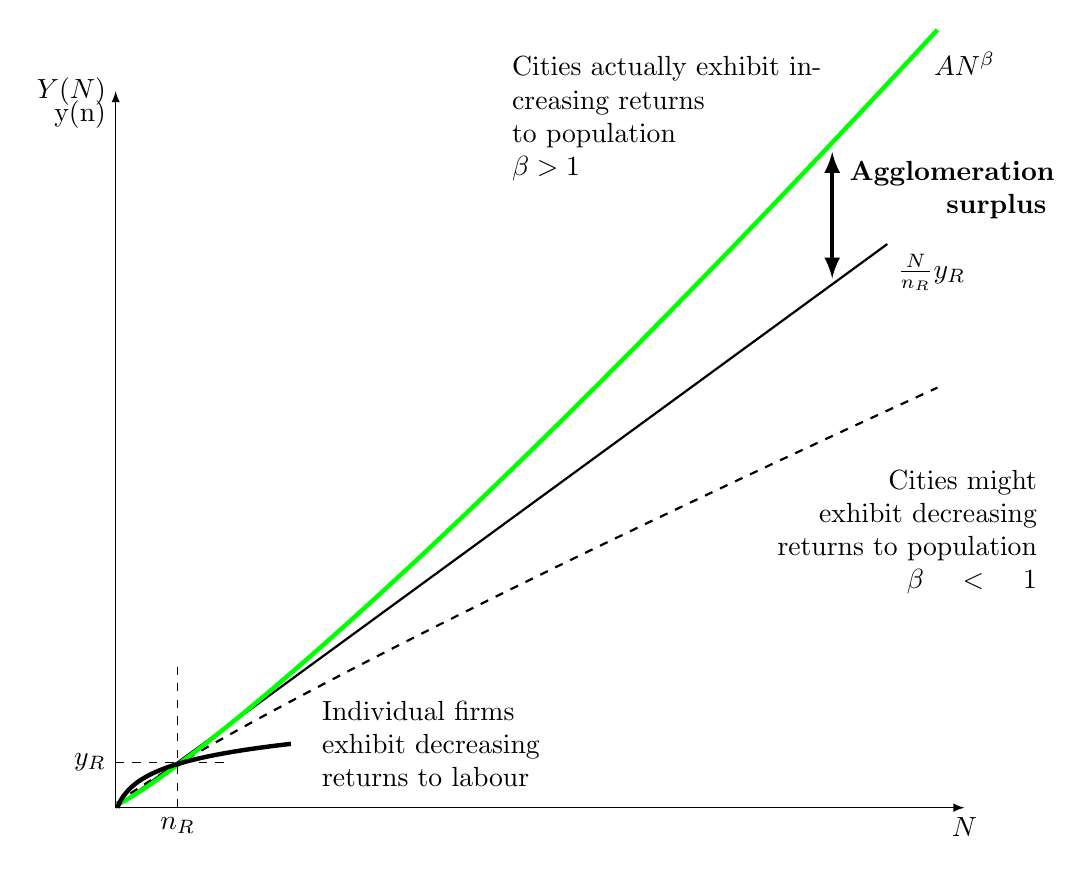
\begin{tikzpicture}[scale=.7, my plot/.style={thick, smooth, samples=100, domain=0.1:2.2},
plot2/.style={thick, smooth, samples=100, domain=0.1:14.99},
                    my grid/.style={dashed,opacity=0.5, every node/.style={black,opacity=1}},
                    my axis/.style={latex-latex}]
 
 \draw[my axis] (0,13)node[left] {$Y(N)$} --(0,0)-- (15.4, 0) node[below] {$N$}; 
%creates the axis 
 \node at (0,13)[below left]{y(n)};
 
\coordinate (origin) at (0,0);
\def\x{0.45}
\def\y{2.1}
\def\b {$15/(2*ln(\y)+.05)$};
%\def\p{0.55} % define the x, y and p )(midpointvalues
%\draw[my plot] (0,0) plot (\x,{ln(\x)});  %Draws curve
%\draw[my plot] (0,0) plot ({\x-.08},{2.3+ln(\x)}); 
\coordinate (Uy) at (\y,{2*ln(\y)+.05});

% THREE SCALE POSSIBILITIES
\draw [thick, ](0,0)--(14, 10.22583)node[below right]{$\frac{N}{n_R}y_R$};   %diagonal line CRS
\draw[plot2, dashed] (0,0) plot ({\x-.08},{(\x)^0.9/1.5 }); %DRS
\draw[plot2, ultra thick, green] (0,0) plot ({\x-.08},{(\x/1.5)^1.15});%
\node at (15.4, 13.5){$AN^\beta$};

%  TEXT
\node at (13.8,12.5) [left, text width=4.5cm]{Cities actually exhibit increasing returns\\ to population\\ $\beta>1$};%IRS
\node at (13.5,5)[text width=4.5cm, align=right] {Cities might\\ exhibit decreasing \\returns to population \\ $\beta<1$};% DRS

% ARROW
\draw[latex-latex, ultra thick] (13, 11.9)--(13, 9.6);
\node at (15.1, 11.2)[ text width=2.5cm, align=right]{\textbf{Agglomeration\\ surplus}};
%\draw[latex-latex] (13, 8.4)--(13, 9.5)node [below right, text width=1.5cm]{\textbf{$\pi$}};

\begin{scope}[ yscale=.75,xscale=1.5]% shift={(1.9,0)} ,
	\coordinate (Uy) at (\y, {2.3+ln(\y)});
  \draw[my plot,ultra thick] (0,0) plot ({\x-.08},{1.15+ln(\x)/2})node[right=.25cm, text width=3.9cm]{Individual firms\\ exhibit decreasing\\ returns to labour}; % production function for generic ferm
	\draw[dashed](.75, 0)node[below]{$n_R$} --(.75, 3.4);
    \draw[dashed](0,  1.1)node[left]{$y_R$} --(1.4,  1.1);
\end{scope}
%
%
%\begin{scope}[shift={(1.9,0)}]
%
% \def\x{0.45}\def\y{2}\def\p{0.55} % define the x, y and p )(midpointvalues
%\draw[my plot] (0,0) plot (\x,{ln(\x)});  %Draws curve
%
%\coordinate (start plot) at (0.6,{ln(0.16)}); % domain start
%\coordinate (end plot) at (10,10); % domain end
%%\draw[my axis] ([shift={(-0.5cm,0.5cm)}]start plot |- end plot) node[left] {$Y(\cdot)$} |- node[coordinate](origin){} ([shift={(0.5cm,-0.5cm)}]start plot -| end plot) node[below] {$L$}; %creates the axis a little 
%
%\coordinate (Ux) at (\x,{ln(\x)}); % set the u(x) coordinate on the curve. Not used
%\coordinate (Uy) at (\y,{ln(\y)}); % set the u(y) coordinate on the curve
%
%\draw [](origin)--(Uy)  ; 
%
%\draw[my grid] (Uy) |- node[below]{$L*$} (origin) |- node[left]{$Y^*$} cycle;%below from on curve, the 
%
%\end{scope}

\end{tikzpicture}

    \caption{While each individual firm exhibits decreasing returns to scale, the city as a whole exhibits increasing returns to scale, and thus produces an agglomeration surplus, $AN^\beta-\frac{N}{n_R}y_R$.}
    \label{fig-agglomeration-surplus} % WAS {fig:Agglomeration-surplus} i think
\end{figure}
% THE FIGURE ILLUSTRATES A GAP IN NEOCLASSICAL PRODUCTION THEORY that we aim to address with this work. THE STRAIGHT LINE IS WHAT NEOCLASSICAL PRODUCTION THEORY PREDICTED. 
 
Our treatment of the urban surplus, which is central to this thesis, is illustrated in Figure~\ref{fig-agglomeration-surplus}. 
% Figure~\ref{fig-agglomeration-surplus} illustrates the increasing returns to urban size. 
\begin{figure}[htb]
    \centering

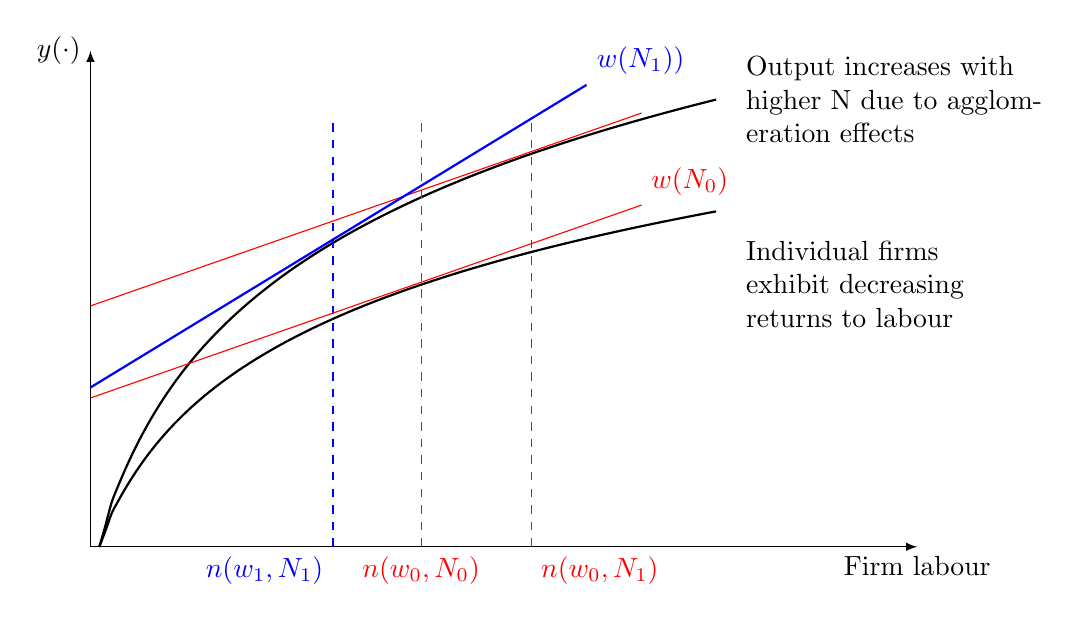
\begin{tikzpicture}[scale=.7, my plot/.style={thick, smooth, samples=100, domain=0.1:1.5},
plot2/.style={thick, smooth, samples=100, domain=0.1:9},
                    my grid/.style={dashed,opacity=0.5, every node/.style={black,opacity=1}},
                    my axis/.style={latex-latex}]
 
 \draw[my axis] (0,9)node[left] {$y(\cdot)$} --(0,0)-- (15, 0) node[below] {Firm labour}; %creates the axis a little 

\coordinate (origin) at (0,0);
\def\x{0.45}
\def\y{2.1}
\def\b {$15/(2*ln(\y)+.05)$};
\coordinate (Uy) at (\y,{2*ln(\y)+.05});


\begin{scope}[ yscale=6, xscale=8]% shift={(1.9,0)} ,
	\coordinate (Uy) at (\y, {2.3+ln(\y)});
  \draw[my plot, thick] (0,0) plot ({\x-.08},{1.15+ln(\x)/2})node[right=.25cm, text width=3.9cm]{Output\ increases\ with\ higher\  N\ due\ to\ agglomeration\  effects}; % production function for generic ferm
\draw[dashed, red](.75, 0)node[below]{$n(w_0, N_0)$} --(.75, 1.3);
\draw[dashed, thin, red](1., 0)node[below right]{$n(w_0, N_1)$} --(1.0, 1.3);
\draw[dashed, blue](.55, 0)node[below left]{$n(w_1, N_1)$} --(.55, 1.3);
\end{scope}

\begin{scope}[ yscale=4.5, xscale=8]% shift={(1.9,0)} ,
	\coordinate (Uy) at (\y, {2.3+ln(\y)});
  \draw[my plot,thick] (0,0) plot ({\x-.08},{1.15+ln(\x)/2})node[below right=.25cm, text width=3.9cm]{Individual firms\\ exhibit decreasing\\ returns to labour}; % production function for generic ferm
\end{scope}

 \draw [thin, red ](0,2.7)--(10, 6.2)node[above right]{$w(N_0)$};   %wage line
  \draw [thin, red ](0,4.37)--(10, 7.87);%node[below right]{$w(N_0)$}; 
  \draw [thick, blue](0,2.89)--(9, 8.38)node[above right]{$w(N_1))$};   %wage line

\end{tikzpicture}

    \caption{Increasing population raises the productivity of workers firm, but is only possible if the wage rises. Firm size may rise or fall}
    \label{fig-wage-workforce-effects} % WAS {fig:Agglomeration-surplus} i think
\end{figure}
% THE FIGURE ILLUSTRATES THE DOUBLE EFFECT OF  INCREASING POPULATION ON FIRM SIZE 
which illustrates how agglomerations might affect returns to scale in the aggregate.
In the lower left, we illustrate a single firm with decreasing returns (DRS) to scale operating at its optimal scale, $n$. The thick diagonal line represents the effect of increasing the number of firms operating at the optimal scale. It is the constant returns (CRS) line. If congestion effects from bringing a large number of firms together were dominant, a city would exhibit decreasing returns to scale,  $N$, and agglomeration would not occur. Research indicates that cities exhibit increasing returns to scale (IRS), illustrated by the upper line, which shows the city generating an increasing surplus as it grows. Even though there are other effects/phenomena, such as congestion as density increases that could theoretically result in cities exhibiting diminishing returns to scale, the evidence suggests that agglomeration effects dominate. The curvature of the line in Figure~\ref{fig-agglomeration-surplus} is determined by an overall  function of the form $N^\gamma$, which we will introduce into in the production function for urban firms.\footnote{The way $N$ enters the firm production function appears to be different from the way it enters the scaling law. We explore the underlying identity below.} 

The empirical \glspl{scaling law} is a feature of urban systems on average across many different contexts.  Empirical work has found %The main conclusion of this literature is the finding of 
scale economies in the range of 3--8 percent (a 10 percent increase in the size of an activity in a city raises productivity in this activity by 0.3--0.8 percent). These agglomeration effects take place both within sectors (localization economies) and between sectors (urbanization economies),  in developed and developing countries, a throughout different historical periods \cite{bettencourtIntroductionUrbanScience2021}. % The results for developing countries are usually similar,  although far less research about agglomeration economies has been conducted in such settings. 
% }
% \vspace{2cm}
 %We will show that they provide a model that can explain economic growth.% If the population rises, the output must rise more than proportionately. %, but if the population responds to the wage premium, the population should then rise. 

The effect of rising agglomeration effects for the firm in our model is ambiguous. Workers are more productive, leading firms to increase employment, but increasing the population requires a higher wage, which negatively affects employment. The result depends quite sensitively on the specific parameterization. We illustrate the two effects in Figure~\ref{fig-wage-workforce-effects}. Fortunately, for our analysis we do not need to know how much population growth goes to existing firms and how much goes to an increase in the number of firms.


\section{Neoclassical growth theories}  \label{section-growth}

Growth theory offers one of the most influential efforts to understand the wealth agglomeration effects established in the scaling and agglomeration literatures.  Growth theory originally focused on identifying the dynamics of macroeconomic systems, and in particular with the implications for the growth of national income. Early models \cite{keynesGeneralTheoryEmployment1937, harrodEssayDynamicTheory1939, domarCapitalExpansionRate1946}  employ a macroeconomic savings function which usually has a fixed savings rate, with savings being reinvested in productive capital. Later models endogenize the savings-investment process. 

The growth models, however, were not spatial models and necessarily abstracted from land rents and distribution. They have nothing to say about the distribution of city products and the effect that distribution might have on growth. When we focus on cities, however, it will become necessary to develop an analysis of city-level saving and investment. %We will do 
IN ORDER TO DO THIS WE DRAW ON SOLOW SWAN APPROACH TO FILLING A SLIGHTLY DIFFERENT GAP IN THE PRODUCTION FUNCTION.

\subsection{The Solow-Swan growth model}

In addition to not being a spatial model, urban growth theory had an important flaw. It did not completely explain the data. % {\color{red} FIX 
The approach taken to address that challenge offers parallels to how we can model urban agglomeration mechanisms.
Existing models of production had described national output as a function of two factors, the national capital and labour stocks. Output should therefore have been completely determined by the growth of those stocks and nothing else. Productivity actually grew more over time than the increases in labour and capital stocks could explain if the production function was correct.

%Solow and others realized it  wasn't working. 
In 1956 Robert Solow \cite{solowContributionTheoryEconomic1956} and Trevor Swan \cite{swanEconomicGrowthCapital1956}
addressed this gap in neoclassical production theory. Solow's paper in particular stimulated a whole literature in the 1960s and launched an entire subfield known as neoclassical growth theory.\footnote{Solow and his contemporaries, including Edward F. Denison \cite{denisonSourcesEconomicGrowth1962}, were attempting to account for the trajectory
of U.S. GDP growth, not to provide a theory of economic development as later theorists were. The distinction, although it does not seem to be commonly drawn, is between quantitative change in the level of GDP and qualitative change resulting from innovation and structural transformations.} %, exploring many variations on the original one-sector structure.  

The \gls{Cobb-Douglas} production function that was in traditional  use neoclassical production theory had been estimated by Cobb and Douglas \cite{cobbTheoryProduction1928} as early as 1928. It had the form
\begin{equation*}
Y=AK^\alpha L^\beta, 
 \label{eqn-Cobb-Douglas}    
\end{equation*}
where $L$ represented the national labour stock, $K$ the national capital stock and  $A$ a convenient scale factor. This \gls{Cobb-Douglas} form captured  important regularities in the cross-sectional national data.\footnote{The function remains the workhorse of growth theory, although later work has found models that preform better e empirically.  A 2021 meta-analysis of 3186 estimates concluded that ``the weight of evidence accumulated in the empirical literature emphatically rejects the Cobb-Douglas specification.''Gechert, Havranek, Irsova, Kolcunova (2021), ``Measuring capital-labour substitution: The importance of method choices and publication bias,'' \cite{GET_REF}. %Review of Economic Dynamics, doi:10.1016/j.red.2021.05.003, S2CID 236400765. 
More sophisticated models such as the CES and translog (TODO WHAT DOES THIS STAND FOR?) functions are now preferred for estimating production functions \cite{GET_REF}.}  % FI
% but the estimates soon showed a systematic bias with time series. 

By the early 1950s it was clear that estimated model parameters were underpredicting output when current levels of national capital and labour stocks were used. Something that was not captured in the initial model was changing over time. The obvious conclusion was that value of the the scale constant $A$  was not constant, it was time-dependent  
 \[Y=A(t)K^\alpha L^\beta.\]
Solow and Swan proposed a way to extend the standard \gls{Cobb-Douglas} production to explain rising productivity over time. 
 %offered a possible explanation for why it would be changing, opening the field for a further series of refinements in an enterprise that became known as `growth theory.' %   R.E. Lucas, Jr., On the mechanics of economic development.}
Solow  argued that ``As a result of exogenous population growth the labour force increases at a constant relative rate'' that we will represent by  $g$:
  \[L(t)= L_0e^{gt}.\] 
If we insert this term into the production function we get a scale term that depends on the changing population 
\begin{eqnarray}
Y &= AK^\alpha (L_0e^{gt})^\beta\nonumber\\
  &= A(e^{gt})^{\beta}K^\alpha L^\beta,
\label{eqn-solow-swan3}
\end{eqnarray}
we see that $A(t)$ can be written
 \[A(t)=Ce^{gt\beta}.\]
transformation provided  the time-dependent term needed to allow the model to track the data better. The model is now known as the \gls{Solow-Swan model}. 

The \gls{Solow-Swan model} correctly predicts the directions of savings and population growth, but not the magnitudes \cite{mankiwContributionEmpiricsEconomic1992}. It successfully explained a good deal of the until-then-unexplained variation over time and between nations. More than half  of the cross-country variation in income, for example,  can be explained by differences in per capita saving (capital) and population growth alone. The estimated influences of saving and population growth with the Solow model appear too large, however. To understand the relationship between saving, population growth, and income, it was necessary to go beyond the  Solow-Swan model.

In the Solow-Swan model growth in productivity is exogenous. By treating economic expansion as exogenously driven, neoclassical growth theory did not explain % could not focus on 
the underlying forces which determine long-run development of nations.   Robert E. Lucas \cite{lucasMechanicsEconomicDevelopment1988} would observe that \begin{quotation}
``[i]t seems to be universally agreed that the model \dots is not a theory of economic development.   \dots while it is not exactly wrong to describe these differences (in GDP  growth rates) by an exogenous, exponential term like A(t), neither is it useful to do so. We want a formalism that leads us to think about individual decisions to acquire knowledge and about the consequences of these decisions for productivity.'' \end{quotation}


The models that followed Solow-Swan, starting with Arrow's 1962 model of `learning by doing' \cite{arrowEconomicImplicationsLearning1962a}, introduced \gls{human capital} and learning in a variety of ways, thus `endogenizing' the growth  process. %This is a central insight. 
This is an important extension. 

Human capital may enter the model as a stock of experience that accumulates in the firm or the sector. It may be proxied by aggregate prior capital investment, as in Arrow's model. The scale term $A$ then becomes $A(K)$.\footnote{The use of capital as the limiting factor formally resembles the Harrod-Domar model \cite{harrodEssayDynamicTheory1939, domarCapitalExpansionRate1946}, although the interpretation is different. Arrow uses capital a a proxy for knowledge, not machinery.} Arrow uses a dynamic interpretation of increasing returns approach  that was perhaps the first to  render technological progress endogenous in a growth model.\footnote{The version of how the field has developed that we present leaves out many who were engaged in and contributing to the evolution of growth theory. The introduction to  Arrow's paper cites several. Spear and Young \cite{spearMACROECONOMICDYNAMICSSURVEY2018} provide a more inclusive overview. It seems clear that neoclassical growth theory was the result of a general ferment in the economic profession, not simply the product of a few pioneering individuals.} 
% {\color{red} 
% and  Levhari  \cite{levhariExtensionsArrowLearning1966} by  the experience of workers,  as in Sheshinski \cite{sheshinskiOptimalAccumulationLearning1967}.
% } 
Other proxies for learning were considered by various authors \cite{levhariExtensionsArrowLearning1966, sheshinskiOptimalAccumulationLearning1967}, incuding the the amount of innovation by other firms and sectors  \cite{kingEndogenousGrowthRole1989}. Sheshinski and Levhari showed that Arrow's formulations was quite general and could incorporate a range of effects as well as different forms for the production function.


To understand  growth theories based on \gls{human capital},  sometimes called `\gls{effective labour},' it is helpful to notice that Solow's formulation is unchanged if we substitute `labour $\times$ skill' for $L$ in his model. Both components of `labour $\times$  skill,' or effective labour grow over time. Output then grows at the same rate as the effective labour supply. Mankiw, Romer and Weil \cite{mankiwContributionEmpiricsEconomic1992} showed that  
Solow's model  augmented by including human capital $H$  fit the data better the unamended Solow-Swan model. Their equation was, in our notation,   
\begin{equation*}
Y=A(t)K^\alpha H^\gamma L^\beta, 
% \label{eqn-mankiw}    
\end{equation*}
where $H^\gamma$ is a form of human capital. (They assume $\alpha+\gamma<1$, which implies decreasing returns to all forms of capital take together.) The apparent effect of increasing labour supply and technological change could be, therefore, the combined effect of rising labour supply, technological change, and increasing labour skill and even agglomeration. Later studies would attempt to disentangle the four components.


%???       It is no surprise that adding a variable allowed the model to track the data better. More  interesting is that the appearance of term $1-\alpha}$ in the scale factor $A$ suggests a spillover effect of human capital on the productivity of other factors.\footnote{Breton, T. R. (2013). ``Were Mankiw, Romer, and Weil Right? A Reconciliation of the Micro and Macro Effects of Schooling on Income'' (PDF). Macroeconomic Dynamics. 17 (5): 1023--1054. doi:10.1017/S1365100511000824. hdl:10784/578. S2CID 154355849.}  

%The estimated model explained 78\% of the variation in income across countries.
% the estimates of $\beta$ implied that\textbf{ human capital's external effects on national income are greater than its direct effect on workers' salaries.}%(\url{https://en.wikipedia.org/wiki/Solow\%E2\%80\%93Swan_model)}.  Theodore Breton provided an insight that reconciled the large effect of human capital from schooling in the Mankiw, Romer, and Weil model with the smaller effect of schooling on workers' salaries. He demonstrated that the mathematical properties of the model include significant external effects between the factors of production because human capital and physical capital are multiplicative factors of production.[20] The external effect of human capital on the productivity of physical capital is evident in the marginal product of physical capital:
%    \[ MPK={\frac {\partial Y}{\partial K}}=\frac {\alpha A^{1-\alpha }(H/L)^{\beta }}{(K/L)^{1-\alpha} }\]

 %Ludcas on the mechanics of ec dev

%, We draw on these models,  formulated at the level of nations, to describe  agglomeration and productivity at the level of cities.% (per Lucas on mechanics), See Burmeister and Dobell (1970) for an excellent introduction and survey. 

%In these models, saving and population growth rates determine the growth trend of the economy. which assumed  diminishing returns to capital and labour separately and constant returns to both factors jointly, 

% MISSED Mankiw et al.equation 
 % The  model became\footnote{Because they work with time series, all the quantities are dated. We omit the time marker for notational simplicity.}

% NOTE for  K   
%If we replace the labour-capital technology of the Solow model with a land-labour technology of the same form, and treat labour as the mobile factor and land as the immobile, we obtain a model that predicts exactly the immigration flows that occurred and for exactly the reason - factor price differentials - that motivated these historical flows

%One of the predictions of the neoclassical growth model, even  when the concept of capital includes human capital, is that without  continuing improvements in technology, per capita income growth eventually ceases on the equilibrium path. 

Identifying  plausible ways that human capital might affect development was relatively easy. However, measurement of human capital presents great practical difficulties. To extract the implications of a particular path, it was also necessary to construct a tractable model, analyze its dynamic properties, and find proxy data to test the initial hypothesis.   A series of papers did exactly that. It is important to note that these models all open the possibility that governments can promote growth through investment in education, research, technology transfer, and incentives for firms.

%{\color{red} In this work, human capital comes in in xx way. --. we integrate parts of these models.. this is what we take from this work..}


%{\color{red} WE STOPPED HERE} 

\subsection{Endogenous (neoclassical) growth models}
A new wave of research on economic growth was stimulated by Romer \cite{romerIncreasingReturnsLongrun1986} and Lucas \cite{lucasMechanicsEconomicDevelopment1988}. In their models, returns to scale are external to single economic agents and internal to a sector or larger parts of the economy. In other words, private decisions by firms or individuals may enhance the productivity of other firms or individuals. This insight is built into our urban models as a growth-enhancing effect of agglomeration. 

%Basically, two branches have developed, pioneered by Romer (1990) and Lucas (1988). CHECK THESE SOURCES

Paul Romer's 1986 model, based on his 1983 thesis \cite{GET_REF}, describes `learning by investment.' In this model, the increase in {total factor productivity} depends on firms' learning, or investment specifically in knowledge accumulation through research, rather than output. He goes on to  explicitly model the decision to invest in the production of knowledge. The production function  can be written
\[Y = A(R^T)R^\gamma  K^\alpha L^\beta, \]
where $R$ is the research effort of the specific firm, and $R^T=\sum_iR_i$ is the total research in the industry,  $R$ is a choice variable for the firm, which is to say, it decides how much to invest in research. The distinctive  feature of this model is the spillover effect on all other firms of the firm's R\&D investment. Economy-wide or  \gls{total factor productivity} is enhanced by individual firms investing in their own productivity. $A(R^T)$. %\textbf{This is the logic of our own model of agglomeration effects in the city.}

In 1988 Lucas also argued that technical progress is endogenous. He proposed a model that is  close technically to the models of Arrow (1962), Uzawa (1965)and Romer (1986). Following our notation, 
\[ Y = A(H^e) K^\alpha (HeL)^\beta \] 
where $H^e$ is the economy's average level of skill (human capital).  Improvements in skill in any firm  increase overall productivity. The compound term, $HeL$,  can be understood as the `effective' labour force of the firm, where $L$ is size of the workforce, $H$ is the skill level of the  workers that the firm hires,  $1-e$ is the fraction of worker time  spent in training, and $e$, is the fraction of work time spent working.\footnote{A feature of this formulation is that $e$ is a choice variable for the firm. It could as easily be a choice variable for workers in the aggregate model.} 
More time training increase $H$ but reduces $e$, so the firm faces a tradeoff between investing time in training and working in firms.
% CHECK NOTATION ***

The difference between Romer style and Lucas style theories is that endogenous growth in the theory of Romer is caused by accumulating technology (or knowledge), which can be called social capital, while in Lucas it is through training, which increases human capital. %\footnote{Although it is not of direct concern for our work, it is useful to recognize that much of the emphasis in these models is on finding the conditions that can explain the observed long-term  and growth over and above that driven by exogenous population or technology growth. } 
Although Romer emphasizes the decisions made by firms while Lucas bases his theory mainly on  decisions by households, both illustrate internal effects of human capital. In one case it whether it is an external or `spillover' increasing the productivity of all firms, in the other it is the individual worker undergoing training to become more productive. 

The evidence supports the existence of significant learning spillovers in a variety of industries. Using survey data, Mansfield (1985) found that information about new processes and products in ten industries surveyed had widely diffused within a year. Spillovers have also been found in econometric studies: Irwin and Klenow (1994) find them in semiconductors; Thornton and Thompson (2001) in wartime shipbuilding; Lieberman (1989) in chemicals; Foster and Rosenzweig (1995) in the adoption of high-yielding seed varieties; and Conley and Udry (2007) in the adoption of best practices by Ghanaian pineapple farmers.\footnote{A model of a national economy that uses the number of urban dwellers would probably track output just as well as one using the number employed as the mainline growth models do. As countries develop, cities account for an ever-increasing share of  national populations and an ever-increasing share of national income.  This is  even more likely when we recall that the principle insights coming out of neoclassical growth theory point to human capital and education as the mystery factor in growth and cities are where the most skilled workers concentrate and where the strongest educational institutions tend to be.} 


\section{Jacobs-style agglomeration effects and the scaling law}\label{section-growth-Jacobs}

Jane Jacobs' work, mentioned above, formulates % introduced 
an alternative but compatible explanation for the increasing productivity that growth theorists tried to explain. She argued that when people come together in cities they make each other more productive \cite{jacobsEconomyCities1969}. In her view the increase in productivity is a result of increasing communication and other network effects between people. % This is a theory of urban agglomeration that can be written for the firm level as%, Remaining with the notation of the growth theorists, it can  be written, 
If we take the relationship implicit in her work, and write it in the language of modern growth theory, we get:

\begin{equation}
y(t) = A_f(L^T,t) K^\alpha L^\beta 
%y(t) = A_f(L^T(t)) K(t)^\alpha L(t)^\beta, 
\label{eqn-production-jacobs}
\end{equation}
where the  lowercase $y$  indicates that Equation~\ref{eqn-production-jacobs} is a \textbf{firm-level}, or micro-economic, formulation. The $L^T$  in the function $A_f$ gives the size of the total urban labour force or urban population.

We impose the standard neoclassical diminishing returns to scale\footnote{$Y(\delta K,\delta L< \delta Y(K,L)$.} assumption on the \gls{Cobb-Douglas} production function, i.e. that 
$\alpha +\beta <1$.  
 %The Cobb-Douglas function used to illustrate these models has the required property.\footnote{To see why, notice that $A(\delta K)^\alpha (\delta L)^\beta = A\delta^(\alpha+\beta) K^\alpha L^\beta$, and $\delta^(\alpha+\beta) <\delta$ for $\delta>1$. } 
 If we then sum across all $F$ firms and assume that all firms are identical we get the \textbf{aggregate} urban production function
\begin{equation}
Y(t) = A(L^T, t)* F *K^\alpha L^\beta. 
\label{eqn-production-jacobs-agg}
\end{equation}
% At the level of the city the aggregate output for this model can be written
% \begin{equation}
% Y(t) = Y_c(L^T(t), t) 
% \label{eqn-production-jacobs-city}
% \end{equation}

If we use consider a fixed capital-labour ratio $d$ as Arrow does,  capital used by the firm is  $K=d*L$ and Equation~\ref{eqn-production-jacobs-agg} becomes
\begin{align}
Y &= A(L^T, t) F d^\alpha L^\alpha L^\beta) \nonumber\\
&=A(L^T, t)F d^\alpha L^{\alpha +\beta} \nonumber\\
&= A(L^T, t) F^{1-\alpha -\beta}d^\alpha * (F L)^{\alpha +\beta} \nonumber \\
&=\bar A(L^T, t) (L^T)^{\alpha +\beta},  
 \label{eqn-production-jacobs-city-2}
\end{align} 
where the  multiplicative constants,  $F^{1-\alpha -\beta}d^\alpha$, are incorporated into the scale factor $\bar A$. 

If we now specify $\bar A$ in Equation~\ref{eqn-production-jacobs-city-2} by: \begin{enumerate}
    \item   assuming that the term $L^T$ enters $\bar A(L^T, t)$ exponentially as in the scaling literature, say as $LT^\delta$,  
    \item defining $Y_0=F K(0)^\alpha L(0)^\beta$, and 
    \item allowing  for additional time dependent growth, $e^{g*t}$,
\end{enumerate}
we can write Equation~\ref{eqn-production-jacobs-city-2} 
\begin{equation}Y_c = Y_0e^{g*t}(L^T)^\gamma. \label{eqn-production-jacobs-scale}
\end{equation}
This is the model commonly used in the scaling literature. We use it as the base for our market model. 



\begin{table}[htb]\small
\centering
\begin{tabular}{|p{1.5cm}|l|l|p{1.5cm}|p{1.4cm}|p{1.cm}|l|p{2.5cm}|}\hline
\textbf{Social Rates} & \textbf{Exponent} & \textbf{Error} & \textbf{Nation} & \textbf{Obser-vations} & \textbf{Year} & \textbf{Unit} & \textbf{Reference} \\ \hline   
GDP             & 1.13 & [1.11, 1.15]  & US           & 363 & 2006        & MSA  & Bettencourt (2013)                 \\ \hline
GDP             & 1.17 & [1.11, 1.22]  & EU           & 102 &             & MA   & Bettencourt  \& Lobo        (2016) \\ \hline
GDP             & 1.22 & [1.17, 1.27]  & China        & 293 & 1996-2014   & prefectural & Zund  \& Bettencourt (2019) \\ \hline
GDP             & 1.14 & [0.98, 1.30]  & India        & 22  & 2011        & UAs  & Sahasranaman \& Bettencourt (2019) \\ \hline
Personal income & 1.1  & [1.03, 1.20]  & Brazil       & 39  & 2010        & MAs  & Breisford et al.  (2017)           \\ \hline
Personal income & 1.35 & [1.19, 1.53]  & South Africa & 8   & 2001        & MMs  & Breisford et al.  (2017)           \\ \hline
\end{tabular}
\caption[Observed scaling exponents]{Observed scaling exponents for urban systems around the world} \label{table-scaling-exponents} (source: Bettencourt \cite{bettencourtIntroductionUrbanScience2021} table 3.1)

\end{table}


To achieve increasing returns at the urban level, it is necessary that the exponents not exceed one, $\gamma=\alpha+ \beta + \delta > 1$.  Empirical  estimates summarized in Table~\ref{table-scaling-exponents} show that this condition is satisfied. These estimates provide a plausible parameter range for modelling. 

%The  model is observationally nearly equivalent to the Arrow model.

% \begin{figure}[!tb]
% \begin{center}
% 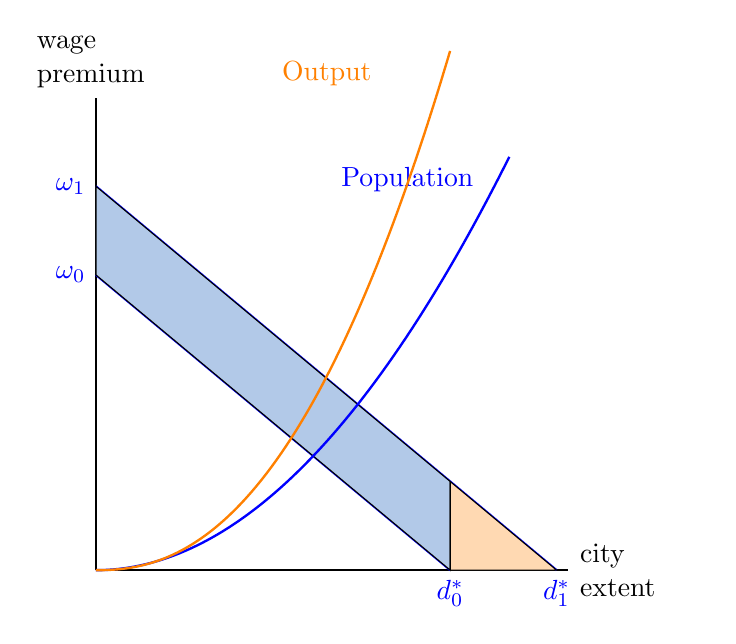
\begin{tikzpicture}[scale=.75]
\def\bndmax{8} 
\tikzset{func/.style={color=blue!80}}	
% EXTENT  BEFORE
\draw[thick](0,0)--(0,8)node[above, text width=1.5cm]{wage \newline premium}; % Y axis
\draw[thick](0,0)--(8,0)node[right=.5, text width=1.5cm]{city\newline extent};  % X axis
%\node at (3.5,-.7){Extent: Walkers};
\draw[thick, blue](0,5)node[left]{$\omega_0$}--(6,0)node[below]{$d^*_0$};
\draw[ thick, blue](0,{5*1.3})node[left]{$\omega_1$}--({6*1.3},0)node[below]{$d^*_1$};
\draw[fill=green!30!blue!30](0,5)--(0,{5*1.3})--(6,5*0.3)--(6,0)--cycle;
\draw[fill=orange!30]({6*1.3},0)--(6,5*0.3)--(6,0)--cycle;
\draw[func, domain=0:7, line width=.3mm,blue, text width=2cm] plot [samples=200] (\x,{\x^2/7})node[below left]{Population};
\draw[func,  domain=0:6, line width=.3mm, orange, text width=2cm] plot [samples=200] (\x,{\x^2.3/7})node[below left]{Output};
%\node[circle,draw=black, fill=white, inner sep=3pt,minimum size=10pt] (b) at (1,2.5) {1};
\end{tikzpicture}
% \end{center}
% \caption[Rising wage and increasing city size]{Rising wage and increasing city size. Agglomeration effects increases the wage premium from $\omega_0$ to $\omega_1$, a higher wage attracts more people to the city, leading to city growth from $d_0^*$ to $d_1^*$, which then begins another cycle of agglomeration and growth }
% \label{fig-rising-wages}
% \end{figure}
% 
\subsection{Dynamics of the Alonzo model with Jacobs agglomeration}
The increase in productivity at the firm level due to agglomeration is the force that drives the formation and growth of cities. In our model, the agglomeration-driven increases in productivity result in an \gls{urban wage premium}. The urban wage premium attracts workers to the city and pays their transportation costs. The size of the wage premium determines the size of the city.

The urban economy modeled this way provides the foundation for our analysis of the urban housing market. We are not attempting to explain the specific process that gives rise to the wage premium: there is strong empirical evidence that it exists, and it is theoretically consistent with the explanations of the growth theories described above. We do need to point to how these agglomeration effects feed into the dynamics of the housing market.

% We do not specify that make urban labour more productive than non-urban labour. % The process has deep historical roots and we do not need to provide an origin story for our project. 
%{\color{red}We can use Figure~\ref{fig-rising-wages} to emphasize the self-reinforcing nature of the mechanism. The blue line  shows population rising as the city boundary moves outward and the orange line shows productivity rising even more quickly due to agglomeration effects. Starting with a city that has grown to size $d_0^*$ based on a wage premium $\omega_0$ in Figure~\ref{fig-rising-wages}, an increase in the productivity due to the various spillover effects discussed in the literature eventually is passed through, at least in part, to the wage raising it to $\omega_1$. }

Conventional microeconomic theory provides us with a rough sketch of the complex process that must occur as agglomeration effects grow. The process will generally be slow, variable, and may involve multiple unsynchronized lags. The basic process, however, is that a firm, discovering its workers are more productive than expected, enjoys unexpected output and profits. Unexpected profits in existing firms will lead to new firms entering the industry. Since the marginal product of each worker is higher than expected, existing firms will want to hire more workers. To do so in a city with full employment, they must raise their wage offers.   The increased wage attracts workers from other firms, putting pressure on them to also increase their wage, so wages rise across the city. The general increase in the wage attracts more workers to the city.

The increase in population will eventually generate additional agglomeration benefits, further increasing wages. At the aggregate level, this positive feedback appears to be solidly supported, but locally, within firms and between firms there will be long and variable lags. Analytical equilibrium models seek to bypass these messy processes, while agent-based models attempt to incorporate them.



%The increase in wages appears as a benefit to workers as workers already in the city. %In Figure~\ref{fig-rising-wages} the area in blue-green represents the worker's share of the increased productivity of the city. 
Assuming that marginal land use per new resident is constant, the city diameter will eventually expand in proportion to the increase in the wage. %, shown as the distance $d^*_0--d^*_1$. Aggregate rent  further expands by the area shown in orange. 
Population increases in proportion to the square of the increase in diameter. %, as  the blue line shows, bu output increases proportionally, as indicated by  the orange line. 

In our model, we connect this agglomeration with financialization through the housing market. The mechanism is that increased wage is translated, with further lags, into rising home prices across the city and rising rental prices for tenants. This means that landowners capture some of the gains due to agglomeration. Owner-occupiers retain the gain and eventually realize it as increased  property values. Financialized owners claim it as rents, and can charge higher rental rates when there is more value to living in the city because of agglomeration effects. % Tenants eventually see the wage gain converted into higher rent payments. 
This flow takes the value created in cities through any mechanism of agglomeration, and captures the flow for finance. 
% Higher home prices and rental rates would be expected to lead to expansion of the housing stock. Adding to the housing stock is a slow process, however, introducing complexities including potentially complex stock and stock-price dynamics. % which we ignore.


% Jacob's view  that rising productivity as a result of urban agglomeration is consistent with the relatively recent research on urban scaling \cite{bettencourtGrowthInnovationScaling2007, loboUrbanScalingProduction2013, bettencourtIntroductionUrbanScience2021, bettencourtOriginsScalingCities2013, kaufmannScalingUrbanAmenities2022, gomez-lievanoStatisticsUrbanScaling2012}.  In section, we show that the firm-level version of Jacobs-style agglomeration in Equation~\ref{eqn-production-jacobs}  
% is equivalent to a \gls{scaling law}. This observation  links the micro-foundation of our model to the macro-economic estimates in the scaling literature. 

% The Jacobs model as we describe it at the level of the firm is 

% The Scaling literature uses  
% \begin{equation}
%     Y=A N^\gamma
% \end{equation}
%This is the function that has been estimated in the scaling literature. 
% The model commonly used in the scaling literature is 
% \[Y = Y_0e^{g*t}N^\gamma\]
% where $Y_0$ is an initial value and $g$ is an exogenous growth rate and $N$ is urban population, which is $L^T$ in our model. The key difference we need to account for is the absence of the firm level of capital and labour in the aggregate function.  %\footnote{Bettancourt (2021) writes the model \[Y_i = Y_0(t)N_i(t)^\beta e^{\xi(t)}\]. Notice that this is similar to the  form that we saw in the \gls{Solow-Swan model} if we substitute $N^\beta$ for Solow's $K^\alpha L^\beta$.  The interpretation is different because the model is used to estimate the parameter $\beta$ and $e^{n(t)}$ is described  as an error term of the form commonly used in estimating multiplicative time-series models.} 


%To show that  Equation~\ref{eqn-production-jacobs} is equivalent to a scaling law we need to  make the synergies that Jacobs points to explicit: we require $L^T$ to generate a spillover effect similar to those  identified in neoclassical growth theory. 
% There are three obvious generic ways to introduce such a term: $L^T$ can augment $A$, $K$, or $L$,

% \begin{align}
%   Y &=\left\{
%     \begin{array}{l}
%      \mathbf{\color{red}(A*L^T)}\quad K^\alpha L^\beta\\
%      A \quad\mathbf{\color{red}(L^T*K)^\alpha} \quad L^\beta\\
%     A K^\alpha \quad \mathbf{\color{red}(L^T* L)^\beta}
%     \end{array}  
%    \right\} \nonumber\\
% \end{align} 
% Each of these produces a firm-level function 
% \begin{equation}%\label{eq-JacobsCobbDouglas}
%  Y=  A(L^T)K^\alpha L^\beta 
% \end{equation}
% \[Y = A*N^\gamma K^\alpha N^\beta= AK^\alpha N^{\beta+\gamma}\]
% \[Y = A (N^\gamma* K)^\alpha  N^\beta= AK^\alpha N^{\beta+\gamma^\alpha}\]
% \[Y = A K^\alpha (N^\gamma* N)^\beta= AK^\alpha N^{\beta+\gamma}\]
% Where $\phi=\beta +\gamma$ or $\beta +\gamma^\alpha$, depending on how the spillover enters. Each of these yields an exponent on $L^T$ that may be greater than one, consistent with both Jacobs and neoclassical growth theory.

% \footnote{It differs from the Solow model in Equation~\ref{eqn-solow-swan3} Where

% \[Y = AK^\alpha \mathbf{\color{red}(L_0e^{g*t})^\beta}L^\beta\nonumber\]
% in that Jacobs, consistent with later literature, assumes that $N$ is endogenous, while Solow assumed an explicit and autonomous time-dependency of $L$.} 

%One more step is needed to produce the standard scaling law: K must be rewritten as a function of employment $N$. The easiest way is to assume as Arrow did that the production process is characterized by fixed coefficients.\footnote{With a Cobb-Douglas function  $K$ will be chosen in a fixed proportion to $L$ at any given wage-capital cost ratio.} $K^\alpha$ is then $cN^\alpha$ for some $c$. Equation~\ref {eq-JacobsCobbDouglas} becomes 



% WHERE TO PUT THIS? \cite{arvidssonUrbanScalingLaws2023} find that cities' tails are responsible for 36--80\% of the observed superlinearities across indicators. 

%will raise the wage, attracting more workers. If they are added in suburbs at the edge of the city (Ricardo's extensive margin) virtually all of the wage premium they receive is dissipated in transportation costs. Closer to the centre,  land rents rise. Owner-occupiers capture the increase as property value appreciation. Tenants are likely to be faced with higher rents.      

%If agglomeration is the source of productivity gains, however, the new workers increase the urban premium, further increasing land values and attracting more workers. 

%The rural population consists of uniformly distributed efficient mix of rural capital producers and workers, all of whom receive $\omega$.%\footnote{This does nothing but fix the price of produced capital in terms of the rural wage.} 

 %Owners of urban firms are  conventional  capitalists, who may earn excess profit if they can capture an unearned surplus from labour.  Any unearned surplus increases the return to urban capital relative to rural capital, resulting in continual expansion of the urban economy. Continuous growth in turn results in continuously rising urban land prices and hence housing costs. We ignore the distributional implications of this feature of the model, and focus instead on the part of value produced by the city that appears as land rent. 

\section{Summary}
% These distinct approaches to understanding agglomeration effects 
% (growth theory  and agglomeration approaches-- which apeare  to be fundamentally different actually produce the same quation, .--)
% We worked through derivations to show how one can be turned into the other. 
% WHENEVER TALKS ABOUT ONE - LOOKS - WHENEVER DIFFERENT INTITIAL POINT AND COME FROM DIFFERENT PLACES the growth  theory all comes out of looking at gdp growth and using the Cobb Douglass to use gdp growth.
% The agglomeration results come out of straight empirical hacking. when xyz and bettencourt go back to how you could get this equation they go back to the Cobb Douglass and that same analysis. -- that's  the logic of that whole chapter one can be turned into the other.

Growth theory, the agglomeration effects identified in Jane Jacob's work, and urban science's empirical work on scaling all produce the same equation. They come from different traditions, draw on different datasets and use different methodologies, but they get to the same place. 
 % all this relationship on why we get growing productivity and it comes to  a certain relationship
In all cases, the reason super-linear scaling of productivity in cities is that the conditions in cities make people more productive. %in cities. The relationship seems to say it's human capital not just the number of workers. %Its their productivity. 
Cities bring people together where they can specialize, get more education, and learn from another. These are all essentially agglomeration effects. 

Agglomeration effects are the third piece needed to build a model relating urban productivity and the financialization of the the urban housing market. % lucas saying - you knowo what jacobs was probably right, that's probably what we've come to with all this work (Lucas is a big  name.)
% Given that there is such a strong theoretical and empirical grounding for urban agglomeration effects in the city, 
We build our model of the housing market on top of a model of the urban system that exhibits positive agglomeration effects.  %***E EDIT THIS. TO CLARIFY RELATIONSHIP BETWEEN SENTENCES. BUILD AGGLOM EFECT INTO MODEL BY EMBEDING SCALING LAW? OR SPECIFICALLY WE EMBED??? 
We model the agglomeration effects by embedding an urban \gls{scaling law} to model how value is create in cities. %to develop the theoretical grounds of our model, we 
% and draw on neoclassical growth theory to explain the growth of national output.
The value created by the scaling effects are the value that financial actors can capture through the financialization of the housing market.